% ****** Start of file OUnoise.tex ******
%%
\documentclass[%
 reprint,
%superscriptaddress,
%groupedaddress,
%unsortedaddress,
%runinaddress,
%frontmatterverbose, 
%preprint,
%showpacs,preprintnumbers,
%nofootinbib,
%nobibnotes,
%bibnotes,
 amsmath,amssymb,
 aps,
%pra,
%prb,
%rmp,
%prstab,
%prstper,
%floatfix,
]{revtex4-1}

\usepackage{graphicx}% Include figure files
\usepackage{dcolumn}% Align table columns on decimal point
\usepackage{bm}% bold math
\usepackage{subcaption}
\usepackage{float}
\usepackage{tikz}
%\usepackage{breqn}
\usetikzlibrary{calc,arrows.meta,positioning}
%\usepackage{hyperref}% add hypertext capabilities
%\usepackage[mathlines]{lineno}% Enable numbering of text and display math
%\linenumbers\relax % Commence numbering lines

%\usepackage[showframe,%Uncomment any one of the following lines to test 
%%scale=0.7, marginratio={1:1, 2:3}, ignoreall,% default settings
%%text={7in,10in},centering,
%%margin=1.5in,
%%total={6.5in,8.75in}, top=1.2in, left=0.9in, includefoot,
%%height=10in,a5paper,hmargin={3cm,0.8in},
%]{geometry}
\DeclareMathOperator\erf{erf}
\DeclareMathOperator\erfc{erfc}
\begin{document}

\preprint{APS/123-QED}

\title{Parameter estimation for correlated Ornstein-Uhlenbeck time-series}

\author{Helmut H. Strey}
 \affiliation{Biomedical Engineering Department and Laufer Center for Physical and Quantitative Biology, Stony Brook University, Stony Brook NY 11794-5281.}%Lines break automatically or can be forced with \\

\date{\today}% It is always \today, today,
             %  but any date may be explicitly specified

\begin{abstract}
\begin{description}
\item[PACS numbers]
May be entered using the \verb+\pacs{#1}+ command.
\end{description}
\end{abstract}

\pacs{Valid PACS appear here}% PACS, the Physics and Astronomy
                             % Classification Scheme.
%\keywords{Suggested keywords}%Use showkeys class option if keyword
                              %display desired
\maketitle

%\tableofcontents
\onecolumngrid
\subsection{Introduction}
In many fields of science we observe time-series of a fluctuating quantitiy: local density fluctuations of a liquid or gas, thermal fluctuations of a bead in an optical trap, thermal fluctuations of soft membranes, or fluctuations of neural activity as measured by fMRI.  In this article, we are exploring how to characterize correlations between two such time-series taking into account that the time series exhibit a relaxation time (memory).  In particluar, we will restrict ourselves to the simplest random process that results in a fluctuating time series with a characteristic relaxation time: the Ornstein-Uhlenbeck (OU) process.  A OU process with mean zero can be expressed by the following Langevin equation:
\begin{equation}
\dot x =  - \frac{k}{\gamma }x + \frac{1}{\gamma }\xi(t)
\label{model}
\end{equation}
where k is the spring constant, $\gamma$ is the friction coefficient and $\xi(t)$ is a randomly fluctuating force.  
We recently published a maximum likelihood method to estimate parameters from an OU process time series, and here we attempt the same for coupled OU processes.
\subsection{Coupled Oscillators}\label{sec_CO}
Here we consider a system of two overdamped oscillators, characterized by a friction coefficient $\gamma$ and spring constant $k$, that are coupled by a spring with a spring constant $c$.  The Langevin equations can be written in the following way:
\begin{equation}
	\begin{aligned}
		\dot{x_1} &= -\frac{k}{\gamma}x_{1}-\frac{c}{\gamma}(x_{1}-x_{2}) +\frac{1}{\gamma}\xi_{1}(t)\\
		\dot{x_2} &= -\frac{k}{\gamma}x_{2}-\frac{c}{\gamma}(x_{2}-x_{1}) +\frac{1}{\gamma}\xi_{2}(t)
	\end{aligned}
\end{equation}
This system can be decoupled by the two eigenfunctions $2y_{1}=x_{1}+x_{2}$ and $2y_{2}=x_{1}-x_{2}$, which results in
\begin{equation}\label{eq_decoupled}
	\begin{aligned}
		\dot{y_1} &= -\frac{k}{\gamma}y_{1} +\frac{1}{\gamma}\xi_{3}(t)\\
		\dot{y_2} &= -\frac{k+c}{\gamma}y_{2} +\frac{1}{\gamma}\xi_{4}(t)
	\end{aligned}
\end{equation}
where $y_{1}(t)$ and $y_{2}(t)$ are two Ornstein-Uhlenbeck processes with different relaxation rates.  The equipartition theorem yields $<y_{1}^{2}> = A_{1} = \frac{k_{B}T}{k}$ and $<y_{2}^{2}> = A_{2} = \frac{k_{B}T}{k+c}$.  The other important relationships are: diffusion coefficient $D=\frac{k_{B}T}{\gamma}$, relaxation times $\tau_{1}=\frac{A_{1}}{D}$ and $\tau_{2}=\frac{A_{2}}{D}$. If the friction coefficients $\gamma$ are different for $x_{1}$ and $x_{2}$ one can still decouple the system of differential equations by finding the eigenvectors and eigenvalues.  For simplicity we assume that both processes have the same friction coefficient or diffusion coefficient $D$.

In many fields, the Pearson Correlation Coefficient $\rho$ is used to characterize the correlation between two time-series.  The connection between our coupling coefficient $c$ and $\rho$ is:
\begin{equation}
	\rho = \frac{\left<x_{1}x_{2}\right>}{\sigma_{1}\sigma_{2}} = \frac{\left<(y_{1}+y_{2})(y_{1}-y_{2})\right>}{\sqrt{\left<(y_{1}+y_{2})^{2}\right>\left<(y_{1}-y_{2})^{2}\right>}} = \frac{\left<y_{1}^{2}\right>-\left<y_{2}^{2}\right>}{\left<y_{1}^{2}\right>+\left<y_{2}^{2}\right>} = \frac{c}{2k+c}
\end{equation}
As expected, for $c=0$ we obtain $\rho=0$, and $c=\infty$ results in $\rho=1$. Often correlation analysis are performed on normalized samples.  It therefore makes sense to define a unitless coupling coefficient $C=c/k$  which can be calculated by estimating $A_1$ and $A_2$ from the data:
\begin{equation}\label{Crho}
	C = \frac{A_{1}-A_{2}}{A_{2}}=\frac{c}{k}
\end{equation}
We can extend this procedure to negative coupling coefficients.  For example, $c=-k$ would results in $\rho=-1$, but at this $c$ (see eq. \ref{eq_decoupled}) $y_2$ becomes unbound.  In order to map the normalized coupling coefficient C in the range from $-\infty$ to $+\infty$ to the Pearson correlation coefficient $\rho=-1$ to $\rho=1$ we suggest the following procedure:  From two normalized samples $x_1$ and $x_2$, we calculate $2y_{1}=x_{1}-x_{2}$ and $2y_{2}=x_{1}-x_{2}$.  From $y_1$ and $y_2$, we estimate the amplitudes $A_{1}$ and $A_{2}$.  If $A_{1}>A_{2}$ then the coupling coefficient $C>0$ and can be calculated using $C=(A_{1}-A_{2})/A_{2}$.  If on the other hand $A_{1}<A_{2}$ then the coupling coefficent is negative and $C=(A_{1}-A_{2})/A_{1}$.  Reversing the process, we can use this procedure to create artificial time-series, by simulating two independent OU processes (eq. \ref{eq_decoupled}) to produce two coupled OU processes $x_{1}=y_{1}+y_{2}$ and $x_{2}=y_{1}-y_{2}$ with a well-defined positive coupling $C$ or $\rho$.  One obtains negative coupling coefficients by using $x_{2}=y_{2}-y{1}$.

\begin{figure}[H]
\begin{center}
\resizebox{.3\textwidth}{!}{%
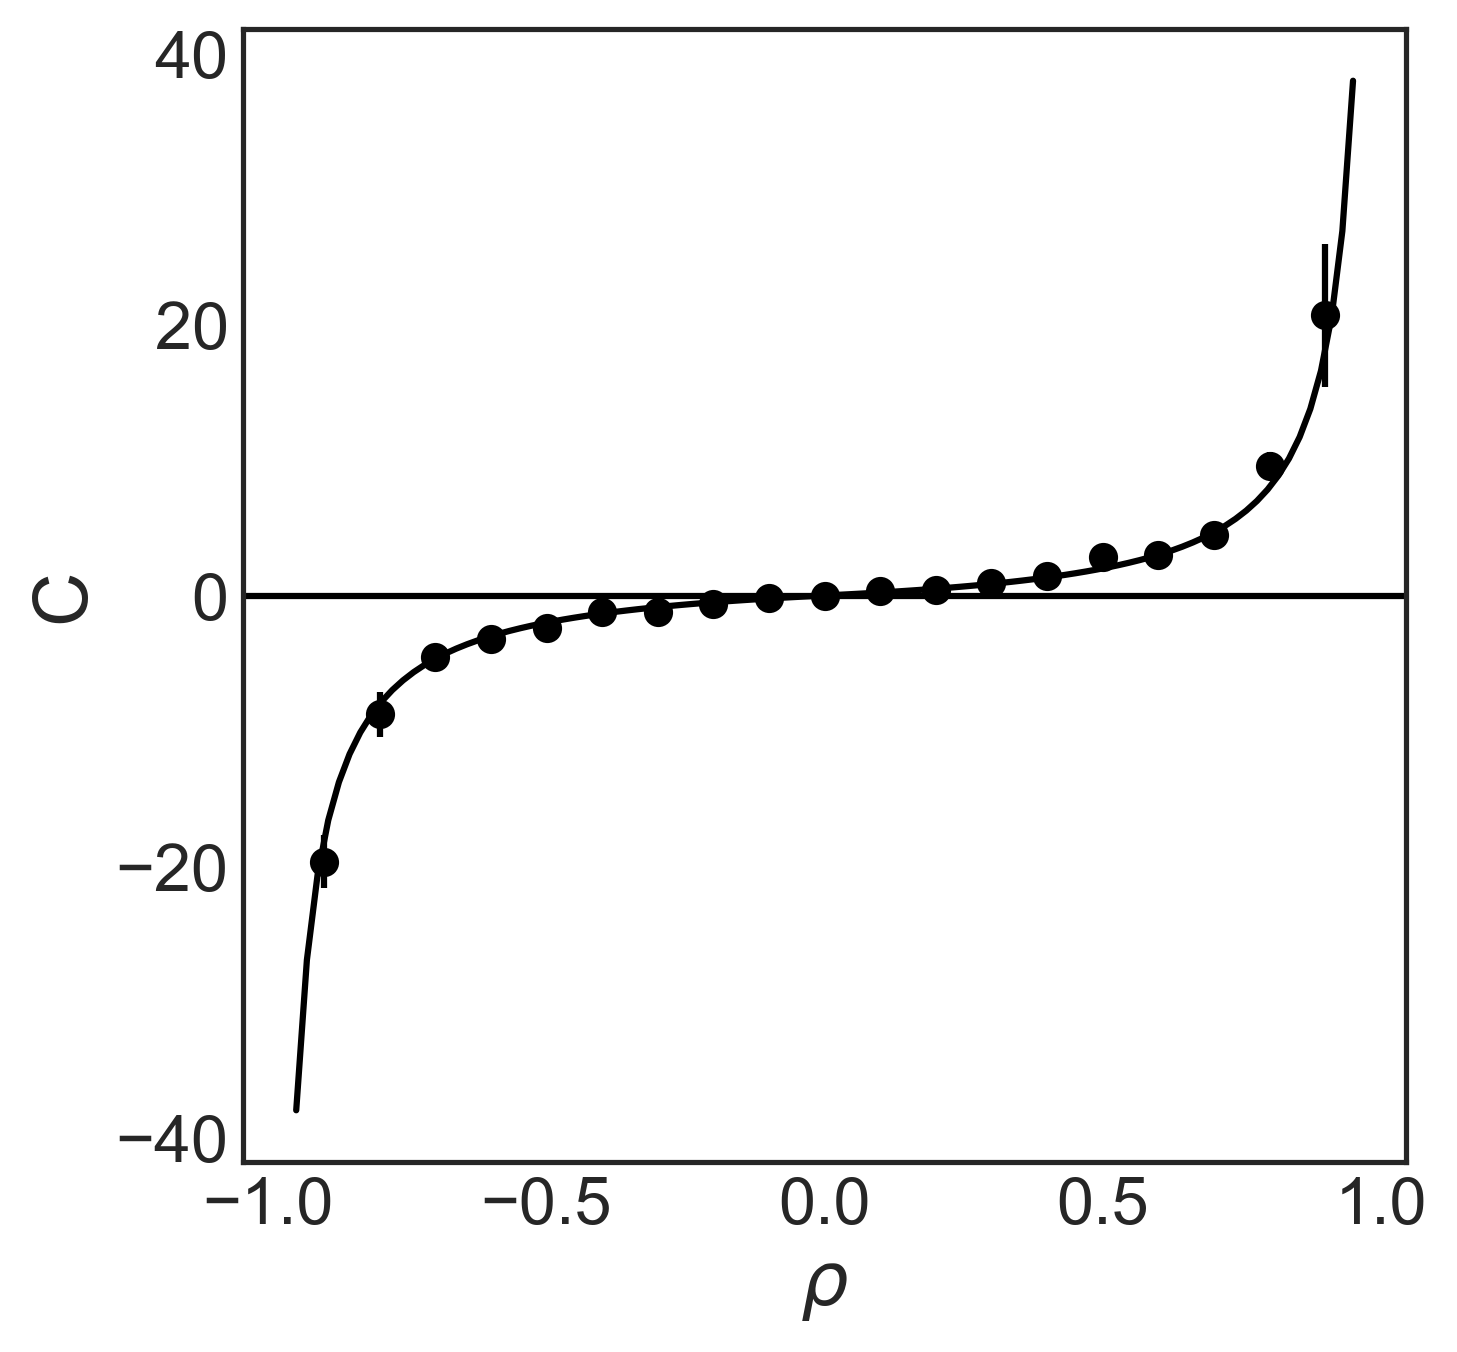
\includegraphics[height=3cm]{corr.png}%
}
\caption{Fig.1: Relationship between coupling coefficient $C$ and Pearson correlation coefficient $\rho$.  The solid line represents eq. \ref{Crho}, whereas the data points represent the parameter estimation by MCMC simulation on artificial data of length $N=1000$.  The errorbars indicate the distribution of estimated $C$s.}\label{fig:corr}
\end{center}
\end{figure}

\subsection{Maximum likelihood solution}
In this section we will express the likelihood of two correlated time-series $x_1$ and $x_2$ in terms of $A_{1}$, $A_{2}$ and $B_{k}\equiv B(\Delta t,D,A_{k})=\exp\left(-\frac{D}{A_{k}}\Delta t\right)$ assuming uniform priors for all parameters.
\begin{eqnarray}
	&&p\left( \left\{x_{1,i}(t_i)\right\},\left\{x_{2,i}(t_i)\right\} \left| D, A_{1},A_{2} \right.\right) \propto
	\frac{1}{\sqrt {2 \pi A_{1}}^{N} }
	\frac{1}{{\sqrt {(1-B_{1}^{2})}^{(N-1)} }}\\
	&&\times\exp \left( -\frac{1}{2A_{1}}\left( {x_{1,1}}^{2} + 
	\sum\limits_{i=1}^{N-1}\frac{ x_{1,i+1}^{2} - 2x_{1,i+1}x_{1,i}B_{1} +x_{1,i}^{2}B_{1}^{2} }{(1-B_{1}^{2})} \right)\right)\nonumber\\
	&&\times\frac{1}{\sqrt {2 \pi A_{2}}^{N} }
	\frac{1}{{\sqrt {(1-B_{2}^{2})}^{(N-1)} }}\\
	&&\times\exp \left( -\frac{1}{2A_{2}}\left( {x_{2,1}}^{2} + 
	\sum\limits_{i=1}^{N-1}\frac{ x_{2,i+1}^{2} - 2x_{2,i+1}x_{1,i}B_{2} +x_{2,i}^{2}B_{2}^{2} }{(1-B_{2}^{2})} \right)\right)\nonumber
\end{eqnarray}
In order to find the maximum likelihood it is convenient to take the logarithm of $p$ and then take the derivatives with respect to $A_{1}$, $A_{2}$ and $D$.
\begin{equation}
\begin{aligned}
	\Phi &= ln \left( p\left( \left\{x_{1,i}(t_i)\right\},\left\{x_{2,i}(t_i)\right\} \left|  D, A_{1},A_{2} \right.\right) \right)\\\\
	&= C - \frac{N}{2} ln(A_{1}) - \frac{N}{2} ln(A_{2})- \frac{N-1}{2}ln \left( 1-B_{1}^{2}\right) - \frac{N-1}{2}ln \left( 1-B_{2}^{2}\right) -\frac{1}{2A_{1}}Q_{1}(B_{1})-\frac{1}{2A_{2}}Q_{2}(B_{2})
\end{aligned}
\end{equation}
with\begin{equation}
	\begin{aligned}
	&Q_{k}(B_{k}) = {x_{k,1}}^{2} + \sum\limits_{i=1}^{N-1}\frac{ {x_{k,i+1}^{2} - 2x_{k,i+1}{x_i}B_{k}} +{x_i}^{2}B_{k}^{2} }{(1-B_{k}^{2})}\\
	&= \frac{x_{k,1}^{2}+x_{1,N}^{2}}{1-B_{k}^2}+\frac{1+B_{k}^2}{1-B_{k}^2}\sum\limits_{i=2}^{N-1}x_{k,i}^{2}-\frac{2B_{k}}{1-B_{k}^2}\sum\limits_{i=1}^{N-1}x_{k,i}x_{k,i+1}
	\end{aligned}
\end{equation}
with $C$ representing an unimportant constant. $Q_{k}(B_{k})$ reveals the fundamental statistic - the only terms that exclusively contain the data $\{x_{k,i}\}$ with $k=1,2$:
\begin{equation}
	\begin{aligned}
		a_{k,EndPoints}&=a_{k,EP}=x_{k,1}^{2}+x_{k,N}^{2}\\
		a_{k,SumSquared}&=a_{k,SS}=\sum\limits_{i=2}^{N-1}x_{k,i}^{2}\\
		a_{k,Correlation}&=a_{k,C}=\sum\limits_{i=1}^{N-1}x_{k,i}x_{k,i+1}\\
	\end{aligned}
\end{equation}
We find the maximum likelihood parameters $A_{k,max}$ and $D_{max}$ by finding the roots of the first derivatives with respect to the three parameters.  The derivative with respect to $A_{k}$ results in the following two conditions:
\begin{eqnarray}\label{partialsigma}
	&&\left.\frac{\partial}{\partial A_{k}}\Phi\right|_{A_{k,max},D_{max}} = -\frac{N}{2A_{k,max}}
	+\frac{1}{2A_{k,max}^{2}}Q(B_{k,max})\\
	&&+\frac{\partial B_{k}}{\partial A_{k}}\left.\left(\frac{B_{k,max}(N-1)}{1-B_{k,max}^2}
	 -\frac{1}{2A_{k,max}}
	 \frac{\partial Q(B_{k})}{\partial B_{k}}
	 \right)\right|_{A_{k,max},D_{max}}=0
\end{eqnarray}
with
\begin{equation}
	\frac{\partial}{\partial B_{k}}Q_{k}(B_{k}) =  \frac{2}{(1-B_{k}^{2})^{2}}\left(B_{k}a_{k,EP}+2B_{k}a_{k,SS}-(1+B_{k}^{2})a_{k,C}\right)
\end{equation}
and
\begin{equation}
	\frac{\partial B_{k}}{\partial A_{k}} = \frac{B_{k}D\Delta t}{A_{k}^{2}}
\end{equation}
The derivative with respect to $D$ can be written:
\begin{eqnarray}\label{partiald}
	&&\left.\frac{\partial}{\partial D}\Phi\right|_{A_{k,max},D_{max}} =\\
	&&\left(\frac{B_{1}(N-1)}{1-B_{1}^{2}}
	-\frac{1}{2A_{1}}\frac{\partial}{\partial B_{1}}Q_{1}(B_{1})\right)\left.\frac{\partial B_{1}}{\partial D}\right|_{A_{1,max},D_{max}}\\
	&&+\left(\frac{B_{2}(N-1)}{1-B_{2}^{2}}
	-\frac{1}{2A_{2}}\frac{\partial}{\partial B_{2}}Q_{2}(B_{2})\right)\left.\frac{\partial B_{2}}{\partial D}\right|_{A_{2,max},D_{max}}=0
\end{eqnarray}
with
\begin{equation}
	\frac{\partial B_{k}}{\partial D} = -B_{k}\frac{\Delta t}{A_{k}}
\end{equation}
From these three equations we need to find $A_{1}$,$A_{2}$ and $D$, which can be done using numerical root finding algorithms that are implemented in standard numerical libraries (e.g. Powell hybrid method implemented in MINPACK \cite{osti_6997568}).  In order to estimate the parameter uncertainties, we need to calculate the Jacobian.  Here the only non-zero terms are: 

\begin{equation}
	\begin{aligned}
		\frac{\partial^{2}}{\partial A_{k}^2}\Phi &= \frac{N}{2A_{k}^{2}} - \frac{Q_{k}(B_{k})}{A_{k}^{3}}
		+ \frac{N-1}{1-B_{k}^{2}}\left(B_{k}\frac{\partial^{2} B_{k}}{\partial A_{k}^{2}}
		+ \left(\frac{\partial B_{k}}{\partial A_{k}}\right)^{2}
		\frac{1+B_{k}^{2}}{1-B_{k}^{2}}\right)
		-\frac{1}{2A_{k}}\frac{\partial^{2}Q_{k}(B_{k})}{\partial A_{k}^{2}}\\
		\frac{\partial^{2}}{\partial A_{k}\partial D}\Phi &= \frac{1}{2A_{k}^{2}}\frac{\partial Q_{k}(B_{k})}{\partial D}
		-\frac{1}{2A_{k}}\frac{\partial^{2} Q_{k}(B_{k})}{\partial A_{k}\partial D}
		+ \frac{N-1}{1-B_{k}^{2}}\left(B_{k}\frac{\partial^{2} B_{k}}{\partial A_{k}\partial D}
		+ \frac{\partial B_{k}}{\partial A_{k}}\frac{\partial B_{k}}{\partial D}
		\left(1+\frac{2B_{k}^{2}}{1-B_{k}^{2}}\right)
		\right)\\
		\frac{\partial^{2}}{\partial D^2}\Phi &=
		\frac{N-1}{1-B_{1}^{2}}\left(B_{1}\frac{\partial^{2} B_{1}}{\partial D^{2}}
		+ \left(\frac{\partial B_{1}}{\partial D_{k}}\right)^{2}
		\left(1+\frac{2B_{1}^{2}}{1-B_{1}^{2}}\right)
		\right)
		+\frac{N-1}{1-B_{2}^{2}}\left(B_{2}\frac{\partial^{2} B_{2}}{\partial D^{2}}
		+ \left(\frac{\partial B_{2}}{\partial D}\right)^{2}
		\left(1+\frac{2B_{2}^{2}}{1-B_{2}^{2}}\right)
		\right)\\
		&- \frac{1}{2A_{1}}\frac{\partial^{2}Q_{1}(B_{1})}{\partial D^{2}}
		- \frac{1}{2A_{2}}\frac{\partial^{2}Q_{2}(B_{2})}{\partial D^{2}}
	\end{aligned}
\end{equation}
with
\begin{equation}
	\begin{aligned}
		\frac{\partial^{2} B_{k}}{\partial A_{k}^{2}} &=B_{k}\left(\frac{D^{2}\Delta t^{2}}{A_{k}^{4}}-\frac{2D\Delta t}{A_{k}^{3}}\right) \\
		\frac{\partial^{2} B_{k}}{\partial A_{k}\partial D} & = \frac{B_{k}\Delta t}{A_{k}^{2}}\left(1-\frac{D\Delta t}{A_{k}}\right)\\
		\frac{\partial^{2} B_{1}}{\partial D^{2}} &= B_{k}\frac{\Delta t^{2}}{A_{k}^{2}}\\
		\frac{\partial^{2} Q_{k}(B_{k})}{\partial A_{k}\partial D} &= 
		\frac{\partial^{2} Q_{k}(B_{k})}{\partial B_{k}^{2}}\frac{\partial B_{k}}{\partial D}\frac{\partial B_{k}}{\partial A_{k}}
		+\frac{\partial Q_{k}(B_{k})}{\partial B_{k}}\frac{\partial^{2} B_{k}}{\partial A_{k}\partial D}\\
		\frac{\partial^{2}Q_{k}(B_{k})}{\partial D^{2}} &= \frac{\partial^{2}Q_{k}(B_{k})}{\partial B_{k}^{2}}\left(\frac{\partial B_{k}}{\partial D}\right)^{2}
		+\frac{\partial Q_{k}(B_{k})}{\partial B_{k}}\frac{\partial^{2}B_{k}}{\partial D^{2}}\\
		\frac{\partial^{2}Q_{k}(B_{k})}{\partial A_{k}^{2}} &= 
		\frac{\partial^{2}Q_{k}(B_{k})}{\partial B_{k}^{2}}\left(\frac{\partial B_{k}}{\partial A_{k}}\right)^{2}
		+\frac{\partial Q_{k}(B_{k})}{\partial B_{k}}\frac{\partial^{2}B_{k}}{\partial A_{k}^{2}}\\
		\frac{\partial^{2}Q_{k}(B_{k})}{\partial B_{k}^{2}} &= \frac{6B_{k}+2}{(1-B_{k}^{2})^{3}}\left(a_{k,EP}+2a_{k,SS}\right)
		-\frac{4B_{k}^{3}+12B_{k}}{(1-B_{k}^{2})^{3}}a_{k,C}
	\end{aligned}
\end{equation}
Using these terms, we can now express the Jacobian as:
\begin{equation} J=
\begin{bmatrix} 
\frac{\partial^{2}}{\partial A_{1}^2}\Phi & 0 & \frac{\partial^{2}}{\partial A_{1}\partial D}\Phi \\
0 & \frac{\partial^{2}}{\partial A_{2}^2}\Phi & \frac{\partial^{2}}{\partial A_{2}\partial D}\Phi \\
\frac{\partial^{2}}{\partial A_{1}\partial D}\Phi & \frac{\partial^{2}}{\partial A_{2}\partial D}\Phi & \frac{\partial^{2}}{\partial D^2}\Phi\\
\end{bmatrix}
\end{equation}
whose negative inverse determines the parameter's covariance matrix $C = -J^{-1}(A_{1,max},A_{2,max},D_{max})$. In order to get a better sense of how the parameter estimation errors behave we can calculate the expectation values of the second derivaties considering $N\rightarrow \infty$: $\left\langle a_{k,EP} \right\rangle=2A_{k}$,$\left\langle a_{k,SS} \right\rangle=(N-2)A_{k}$, and $\left\langle a_{k,C} \right\rangle=(N-1)A_{k}B_{k}$.
\subsection{Validation by Simulation}
In this section, we create artifical correlated time-series employing the method mentioned in \ref{sec_CO} to validate our Maximum-Likelihood method against parameter estimation by Markov-Chain Monte-Carlo methods.  For the following plots, we created 400 correlated time-series pairs for Pearson Correlation coefficients of $0.9$, $0.5$ and $0.25$ for $N=1000$ and $N=10000$.  Since the problem is symmetric with respect to the sign of the correlation coefficient we don't need to simulate negative correlation coefficients.

\begin{acknowledgments}
We wish to acknowledge funding by the 
\end{acknowledgments}
\bibliography{correlations}
\end{document}
